\documentclass[11pt]{report}
\usepackage[spanish]{babel}
\usepackage[utf8]{inputenc}
\usepackage{graphicx}
\usepackage{geometry}
\usepackage{fancyhdr}
\usepackage{amsmath}
\usepackage{helvet}
\usepackage{titlesec}
\usepackage{setspace}
\usepackage{tocloft}
\usepackage{hyperref}
\usepackage{csquotes}
\usepackage{placeins}

\setlength{\parskip}{0.5em}

\usepackage[style=numeric,sorting=none]{biblatex}
\addbibresource{referencias.bib} 

\onehalfspacing
\renewcommand{\familydefault}{\sfdefault}

\geometry{
  letterpaper,
  left=3cm,
  right=2cm,
  top=2.5cm,
  bottom=2cm,
}

\addto\captionsspanish{
  \renewcommand{\contentsname}{Índice}
}
\renewcommand{\cftchapdotsep}{\cftdotsep}  % Para capítulos
\renewcommand{\cftsecdotsep}{\cftdotsep}   % Para secciones
\renewcommand{\cftsubsecdotsep}{\cftdotsep} % Para subsections

\titleformat{\chapter}[display]
  {\normalfont\Large\bfseries}
  {\chaptername\ \thechapter}
  {10pt}
  {\huge}
\titlespacing*{\chapter}{0pt}{-20pt}{20pt}  % Ajusta el espaciado aquí

\begin{document}

% Title page
\begin{titlepage}
	\begin{center}
		
\includegraphics[width=0.4\textwidth]{imagenes/logo_ubb.png}\\
		\normalsize FACULTAD DE INGENIERÍA\\
		DEPTO. INGENIERÍA ELÉCTRICA Y ELECTRÓNICA\\[2cm]

		\LARGE \textbf{``Implementación de un Controlador FOC para Motores Brushless con Encoder Utilizando STM32''}\\[6cm]

		\normalsize AUTOR:\\
		RODRIGO FUENTES PEDREROS\\
		\href{https://www.youtube.com/watch?v=dQw4w9WgXcQ}{\phantom{ASDF}}\\[2cm]

		SEMINARIO PARA OPTAR AL TÍTULO DE\\
		INGENIERO DE EJECUCIÓN EN ELECTRÓNICA\\[1cm]

		CONCEPCIÓN - CHILE\\
		AÑO 2024\\
	\end{center}
\end{titlepage}

% Back title page
\begin{titlepage}
	\begin{center}
		
\includegraphics[width=0.4\textwidth]{imagenes/logo_ubb.png}\\
		\normalsize FACULTAD DE INGENIERÍA\\
		DEPTO. INGENIERÍA ELÉCTRICA Y ELECTRÓNICA\\[2cm]

		\LARGE \textbf{``Implementación de un Controlador FOC para Motores Brushless con Encoder Utilizando STM32''}\\[5cm]

		\normalsize AUTOR\\
		RODRIGO FUENTES PEDREROS\\[3cm]

		\large PROFESOR GUÍA:\\
		\large ANGEL ERNESTO RUBIO\\[1cm]
		\large PROFESORES GUÍA ADJUNTO:\\
		\large PEDRO MELIN COLINA
	\end{center}
\end{titlepage}

\normalsize
\pagenumbering{arabic}
\setcounter{page}{3}

\newpage
\tableofcontents

%\newpage
%\listoffigures

%\newpage
%\listoftables

\newpage
\chapter*{Resumen}
\addcontentsline{toc}{chapter}{Resumen}

\newpage
\chapter{Introducción}
\section{Introducción general}
Cuando se habla de motores eléctricos de corriente continua, los motores sin escobillas destacan por su alto desempeño, siendo la opción preferida en aplicaciones como vehículos eléctricos, drones, robótica avanzada y robótica industrial.

Para los motores \textit{brushless}, existe una gran variedad de técnicas de control. Algunas de las más relevantes son el control trapezoidal, utilizado mayormente en drones; el control directo de torque (DTC), empleado principalmente en motores de media y alta potencia; y el control FOC, que se aplica mayormente en robótica. En este documento, se tratará únicamente esta última técnica.

Existen tres aspectos clave que diferencian cada técnica: el rizado de torque, el costo computacional y la complejidad del hardware necesario para su ejecución. En estos aspectos, el control FOC es uno de los que produce menor rizado de torque, aunque requiere un mayor coste computacional y hardware especializado.

Este proyecto presenta la implementación y validación de un controlador de campo orientado (FOC) para motores sin escobillas de corriente continua (BLDC). Se desarrolló la placa controladora utilizando STM32 y se implementó el algoritmo de control FOC en lenguaje C.

\newpage
\section{Marco teórico}
\subsection{Motores \textit{brushless}}
Los motores \textit{brushless}, o motores sin escobillas de corriente continua (BLDC), son un tipo de motores trifásicos síncronos que utilizan imanes permanentes en el rotor y bobinas en el estátor, el cual está formado por un núcleo de hierro laminado. A diferencia de los motores de corriente continua con escobillas, los BLDC no emplean elementos mecánicos para conmutar la corriente en las bobinas. En su lugar, esta conmutación se realiza mediante un controlador electrónico \cite{frick2018bldc}, eliminando el rozamiento y el desgaste asociados a las escobillas, lo que mejora la eficiencia del sistema.

\begin{figure}[ht]
	\centering
	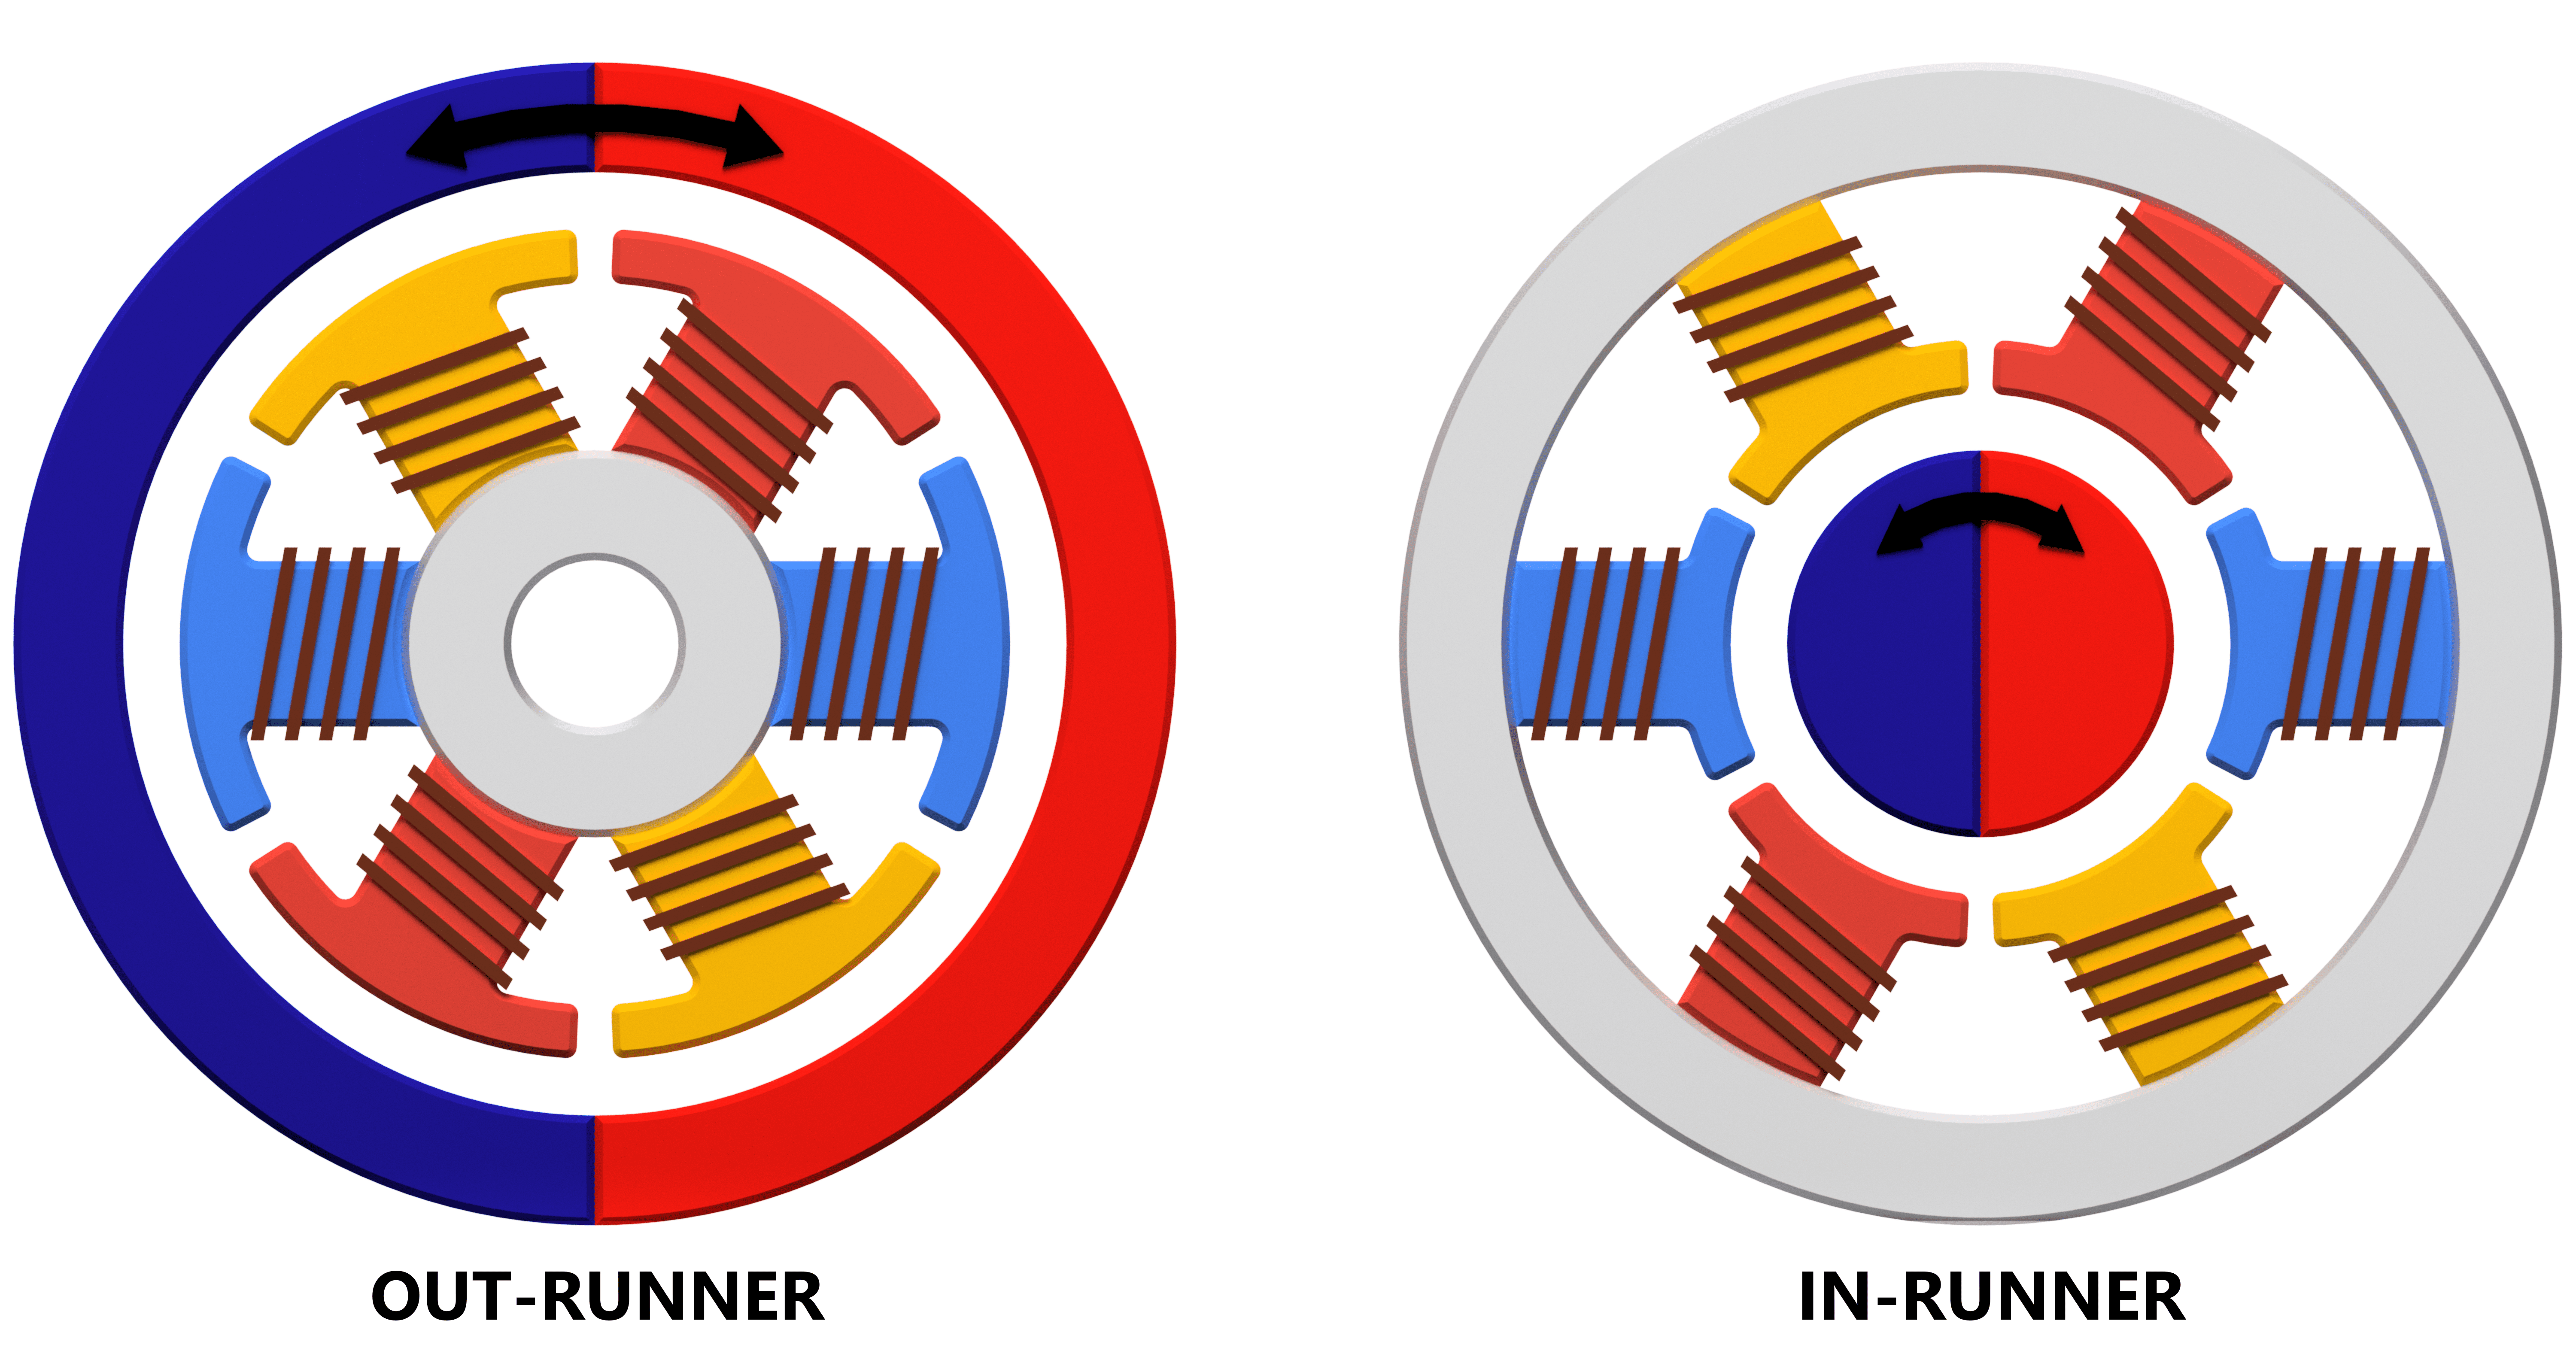
\includegraphics[width=0.6\textwidth]{imagenes/OUT_IN_BLDC_SF}
	\caption{Esquema de motores sin escobillas (\textit{BLDC}).}
	\label{fig:motor_sin_escobillas}
\end{figure}
\FloatBarrier

Similar a los motores trifásicos de corriente alterna, estos pueden tener configuraciones de bobinado en delta o estrella \cite{Millet2022}. Además, pueden presentar configuraciones \textit{in-runner}, donde los imanes están en el centro del eje con las bobinas en el exterior, o configuraciones \textit{out-runner} , donde los imanes se encuentran por fuera del motor, mientras que las bobinas están en el centro \cite{9774372}. Estos motores, al requerir una sincronización entre el campo magnético del estátor y el campo magnético del rotor, suelen utilizar encoders o sensores de efecto Hall para obtener información sobre la posición del eje y, de este modo, mantener una conmutación adecuada. No obstante, también es posible emplear técnicas \textit{sensorless} (sin sensor) para estimar la posición del rotor sin necesidad de sensores físicos. \cite{Gualtieri2018_STEP}

Los \textit{BLDC} se destacan por ofrecer una mayor densidad de potencia, mayor torque, mejor eficiencias y pueden llegar a velocidades mas altas. Sin embargo, al requerir de un controlador electrónico que se encargue de la conmutación para generar el movimiento del rotor, la complejidad y los costos asociados a su implementación son mayores. \cite{AN885}

\newpage
\subsection{Control Orientado de Campo (FOC)}
El control orientado de campo se basa en desacoplar el flujo electromagnético del par motor, permitiendo el control independiente de cada uno. Este desacoplamiento se logra mediante la transformación de las variables trifásicas del motor, que están en un marco de referencia estacionario \(ABC\), hacia un marco de referencia rotatorio \(dq\) que gira síncronamente con el rotor. \cite{power_conv_14}

\begin{figure}[ht]
	\centering
	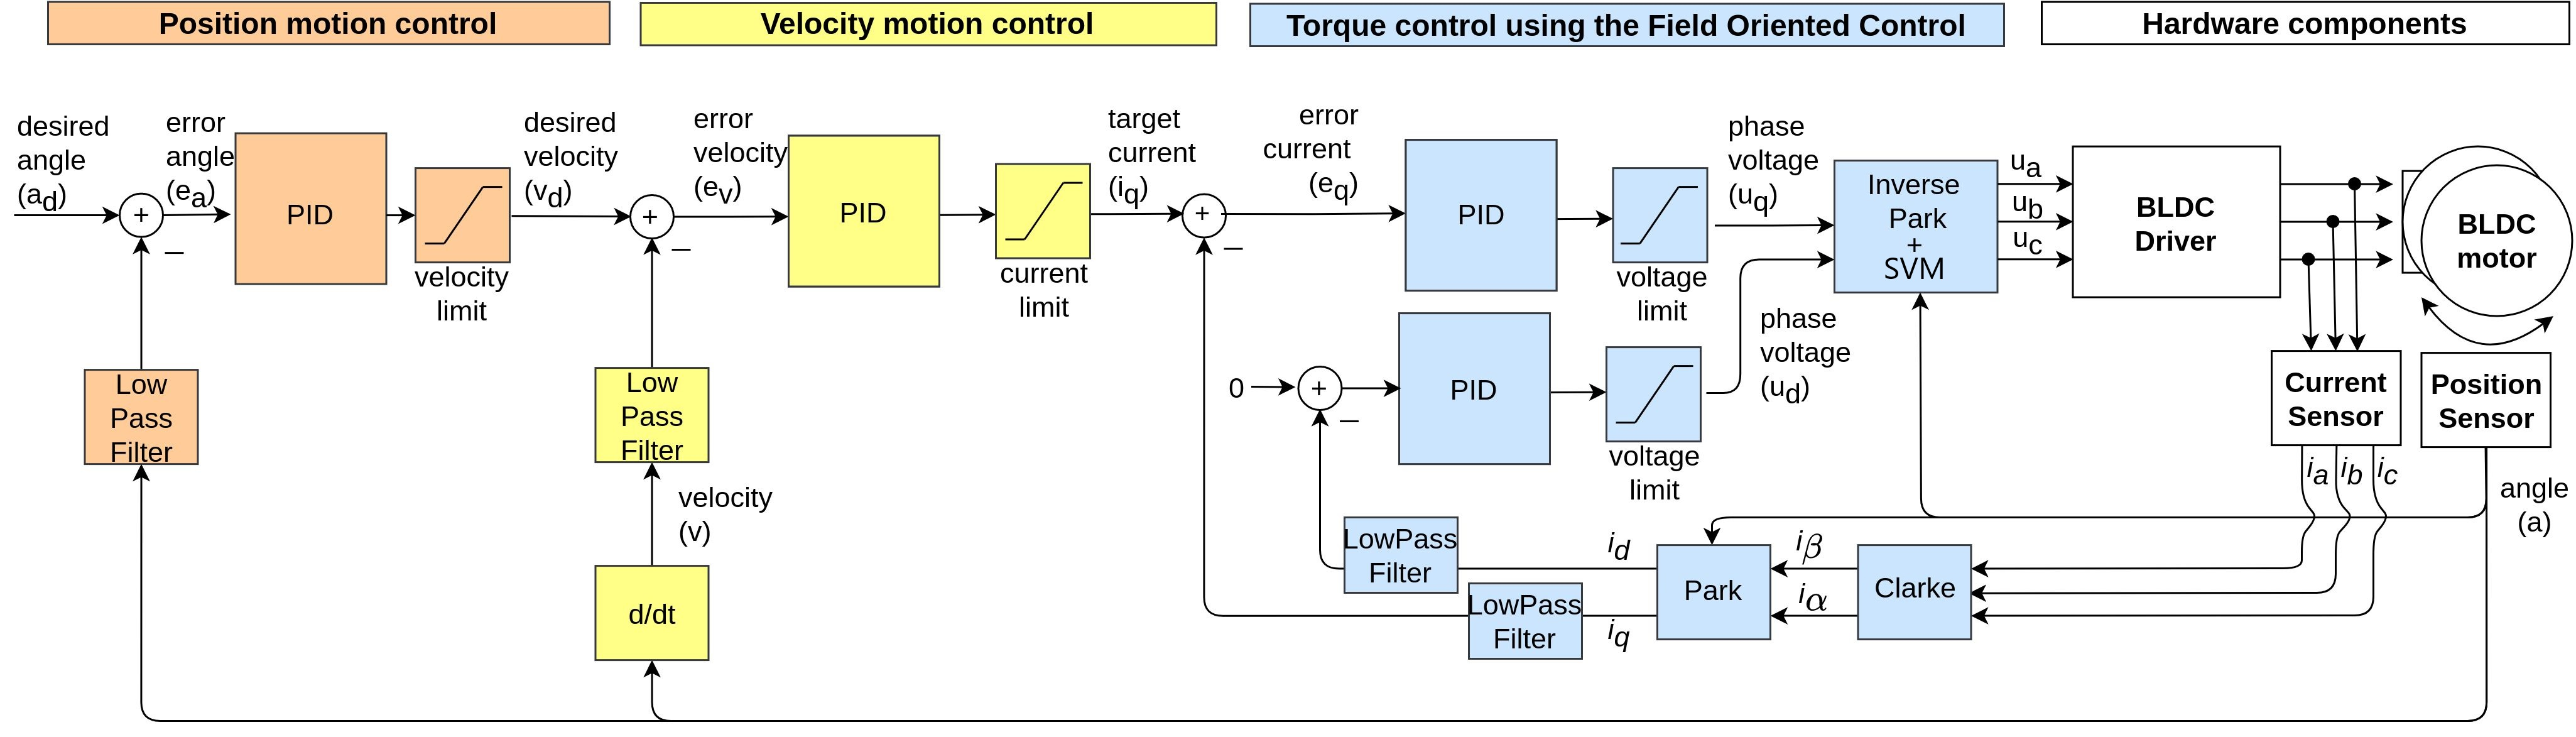
\includegraphics[width=0.9\textwidth]{imagenes/simpleFOC.jpg}
	\caption{Diagrama de flujo del control FOC.\cite{Skuric_SimpleFOC_A_Field_2022}}
	\label{fig:foc_transform}
\end{figure}
\FloatBarrier

La transformación entre los marcos de referencia se realiza aplicando la transformada de Clarke y la transformada de Park. De esta forma, las variables que presentan un comportamiento oscilatorio en el tiempo se convierten en variables de corriente continua, lo que permite emular, en cierta medida, el funcionamiento de un motor con escobillas a nivel de controladores. \cite{power_conv_14}

\subsection{Transformada de Clarke}
La transformada de Clarke convierte un sistema trifásico de corrientes \(ABC\) en un sistema bifásico \(\alpha\beta\), proyectando las corrientes en un sistema de coordenadas bidimensional estacionario. Esta transformación simplifica el análisis al reducir las tres corrientes de fase a dos componentes ortogonales, manteniendo la información esencial del sistema original. \cite{AN1078}


\begin{figure}[ht]
	\centering
	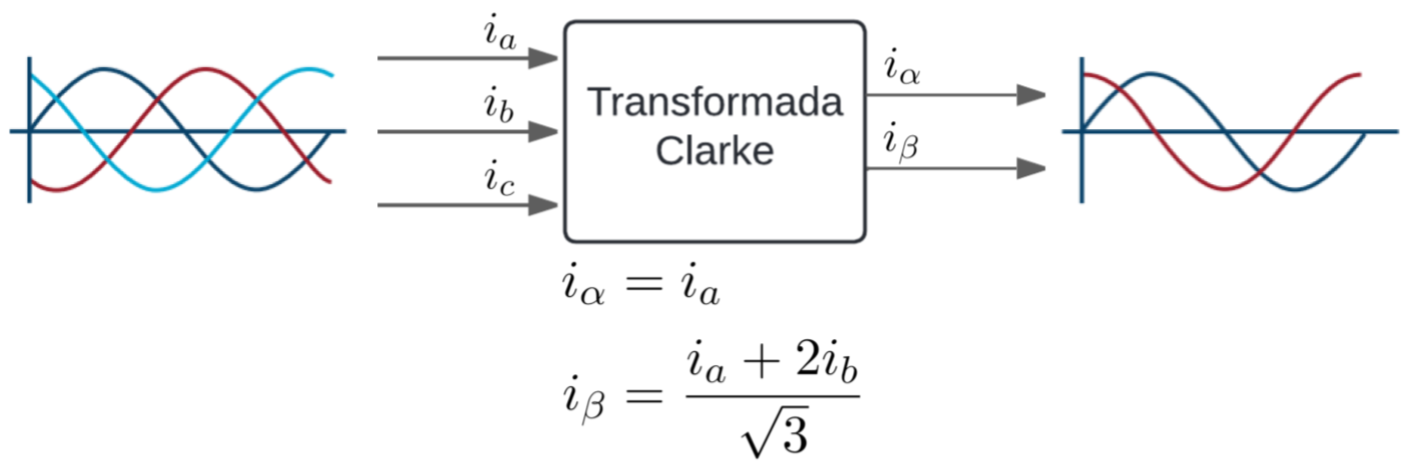
\includegraphics[width=0.8\textwidth]{imagenes/clarke.png}
	\caption{Esquema transformada de Clarke.}
	\label{fig:clarke_transform}
\end{figure}
\FloatBarrier

\newpage
\subsection{Transformada de Park}
La transformada de Park convierte el sistema en el marco de referencia estacionario \(\alpha\beta\) en el sistema en el marco de referencia rotatorio \(dq\) sincronizado con el rotor del motor. \cite{AN1078}

\begin{figure}[ht]
	\centering
	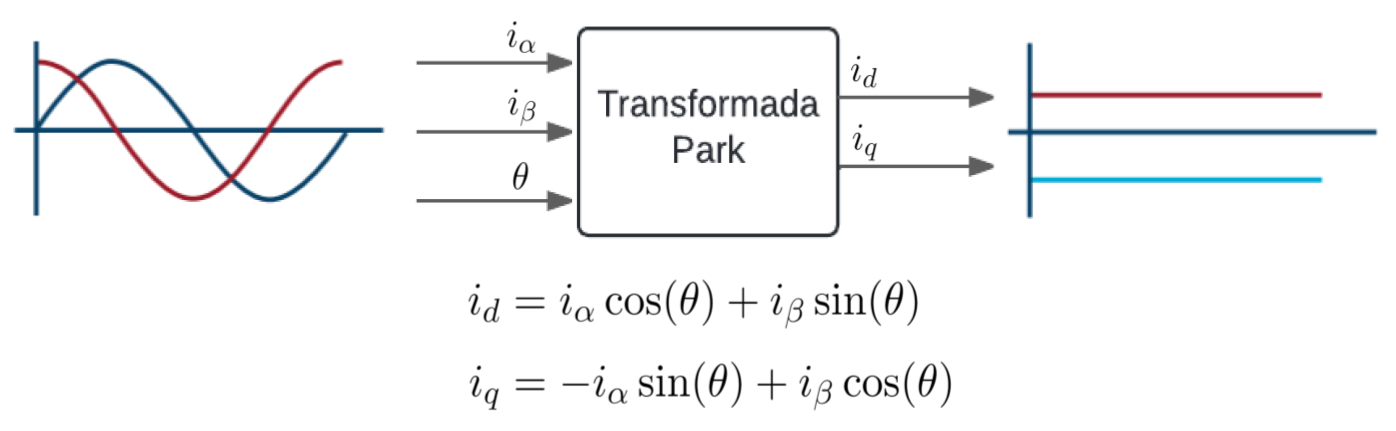
\includegraphics[width=0.8\textwidth]{imagenes/park.png}
	\caption{Esquema transformada de Park.}
\end{figure}
\FloatBarrier

\subsection{Transformada inversa de Park}
La transformada inversa de Park convierte el sistema en el marco de referencia rotatorio \(dq\) de vuelta al marco de referencia estacionario \(\alpha\beta\). \cite{AN1078}.

\begin{figure}[ht]
	\centering
	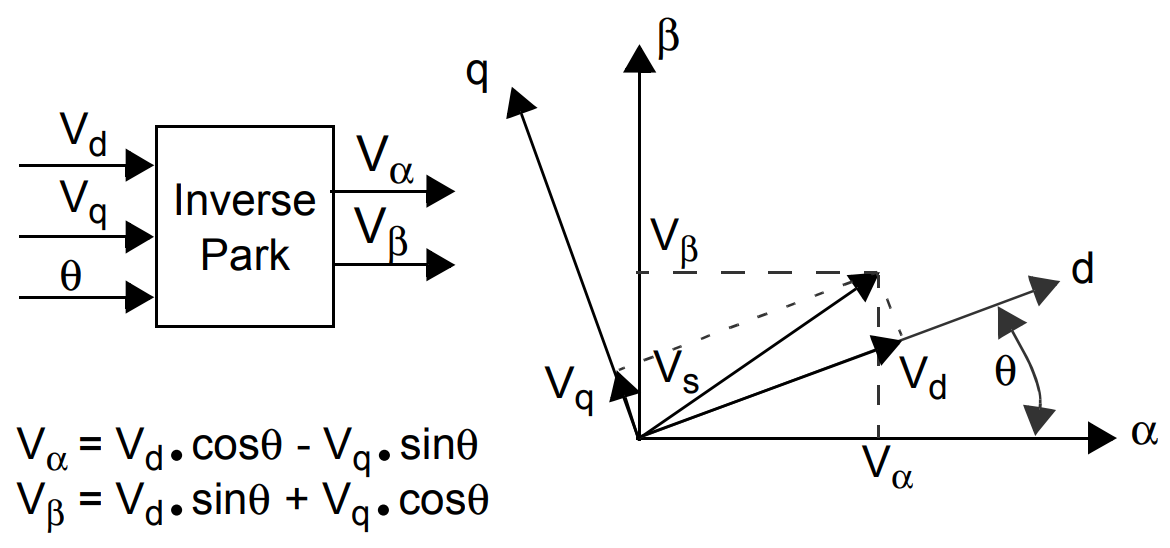
\includegraphics[width=0.8\textwidth]{imagenes/park_inv.png}
	\caption{Esquema transformada inversa de Park.}
\end{figure}
\FloatBarrier

\newpage
\subsection{Modulación de Espacio Vectorial (SVM)}
La Modulación por Vector Espacial (SVM) es una técnica utilizada para el control digital de inversores de voltaje. Representa los estados de conmutación del inversor como vectores de voltaje en el plano $\alpha$-$\beta$, formando un hexágono regular dividido en seis sectores o sextantes.

\begin{figure}[ht]
	\centering
	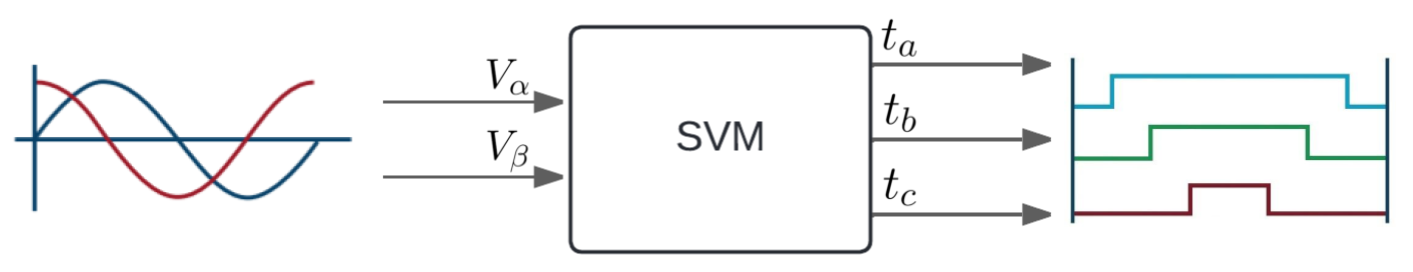
\includegraphics[width=0.6\textwidth]{imagenes/SVM.png}
	\caption{Esquema SVM.}
\end{figure}
\FloatBarrier

Esta técnica busca sintetizar el vector de referencia $\mathbf{V}_{\text{ref}}=(V_{\alpha},V_{\beta})$ mediante una suma ponderada de los vectores de voltaje adyacentes en el sextante donde se encuentre, logrando una aproximación más precisa de la señal deseada.

\begin{figure}[ht]
	\centering
	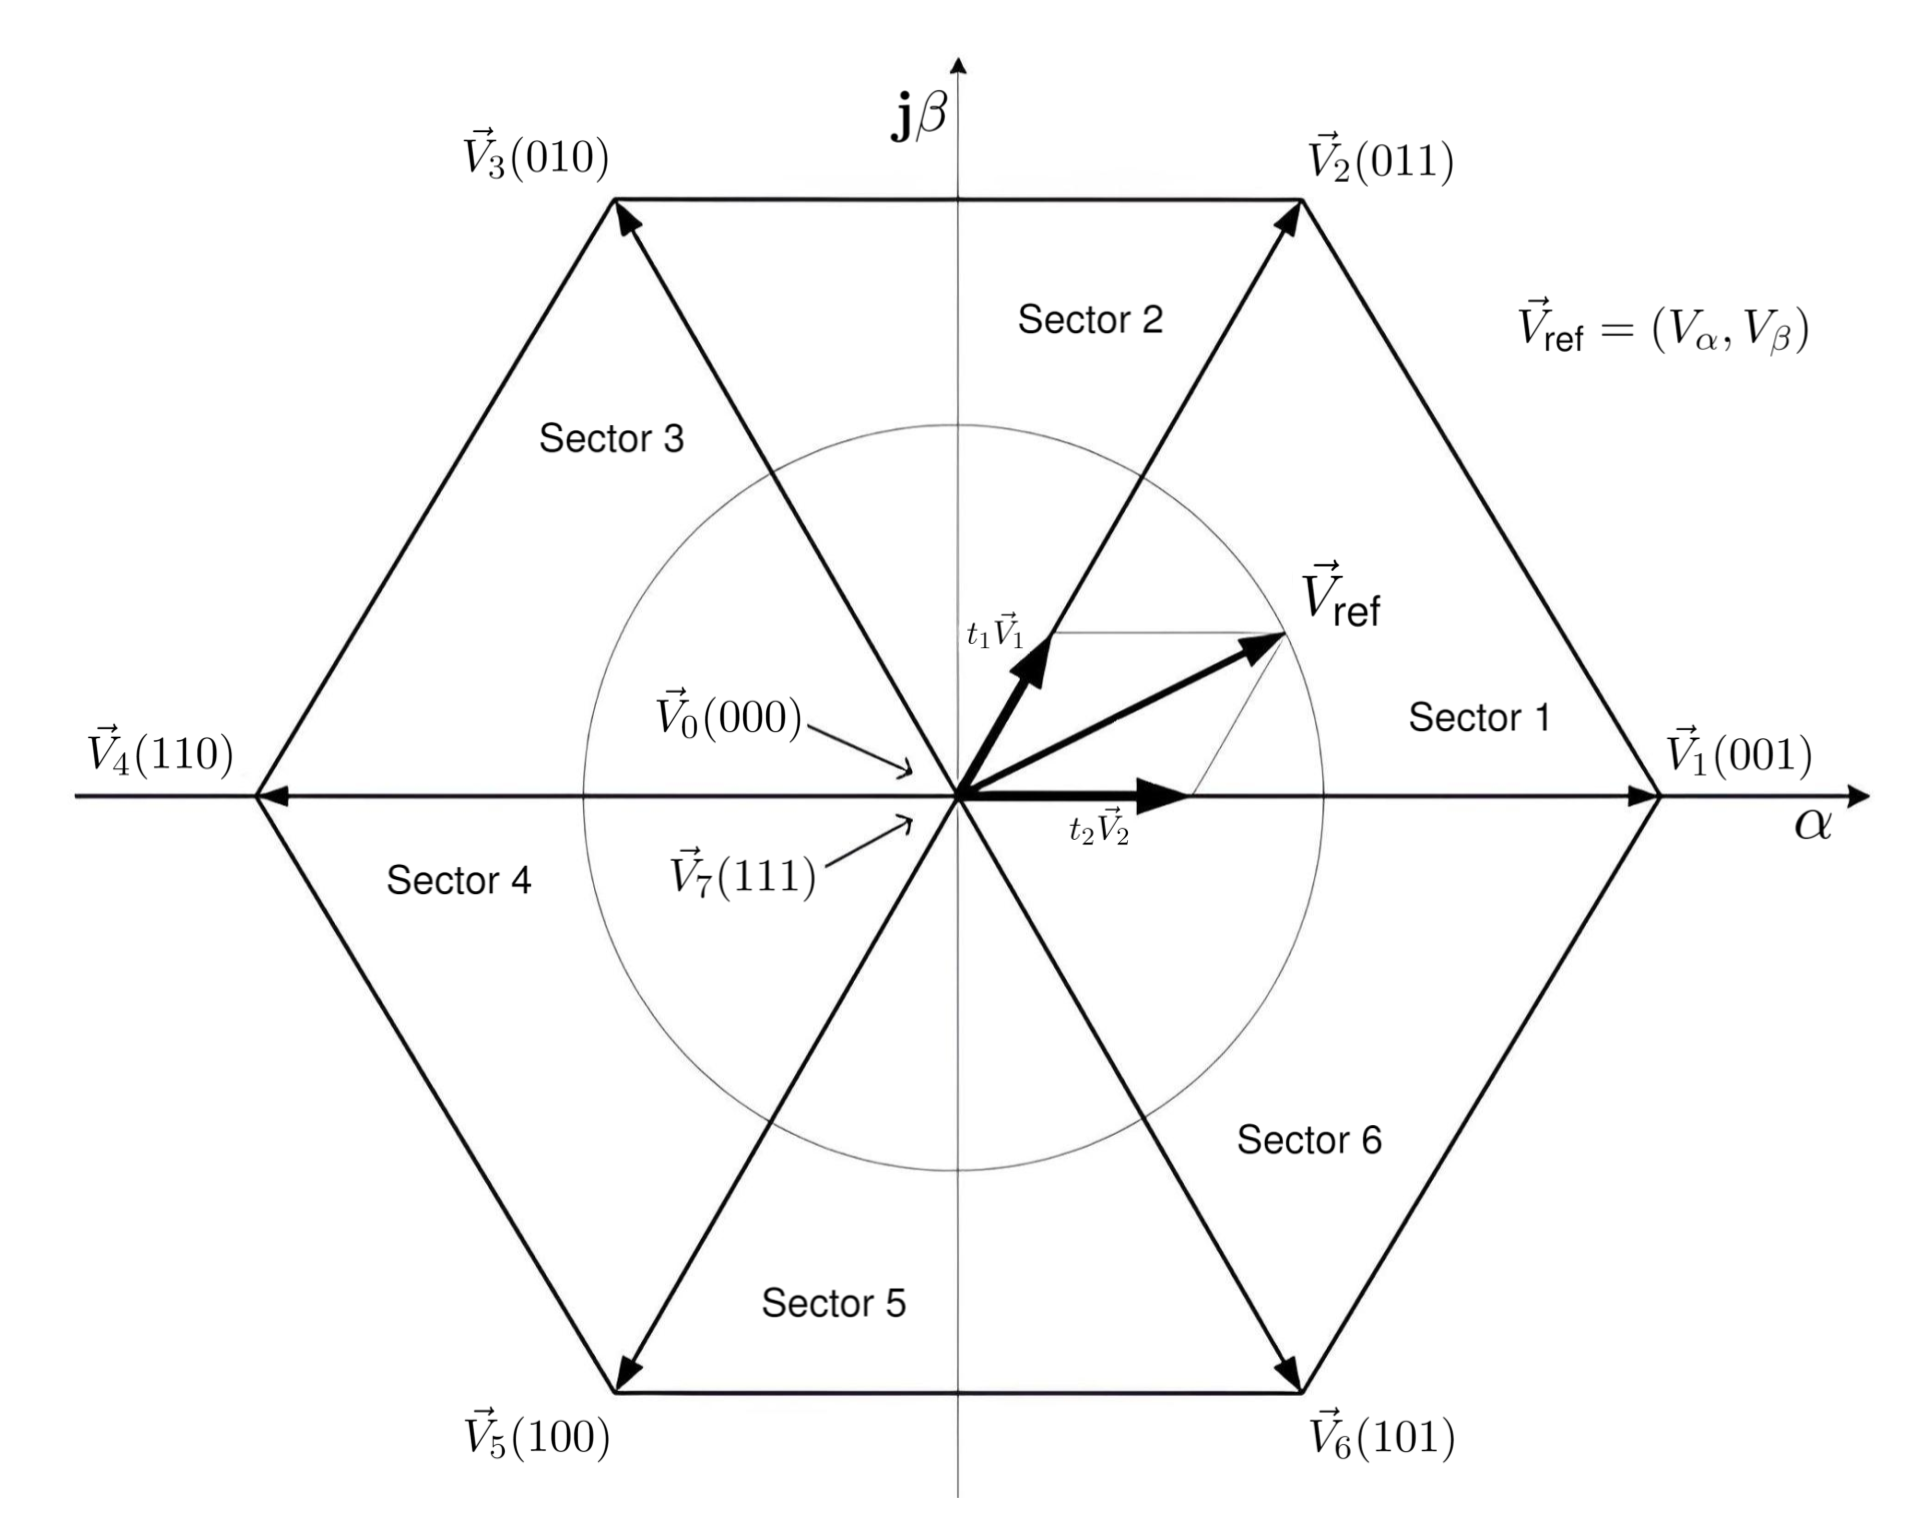
\includegraphics[width=0.5\textwidth]{imagenes/sectantes.png}
	\caption{Sextantes en SVM.}
\end{figure}
\FloatBarrier

Se utiliza un patrón de activación específico que permite minimizar la frecuencia de conmutación de los transistores, aprovechando estados redundantes para reducir las pérdidas asociadas a la conmutación y mejorar la eficiencia del sistema. \cite{power_conv_06}

\begin{table}[htbp]
	\centering
	\caption{Secuencia de Conmutación en SVM}
	\begin{tabular}{ c c c c c c c c }
		\hline
		\textbf{Sector} & \textbf{1}       & \textbf{2}       & \textbf{3}       & \textbf{4}       & \textbf{5}       & \textbf{6}       & \textbf{7}       \\
		\hline
		I               & $\vec{V}_0(000)$ & $\vec{V}_1(100)$ & $\vec{V}_2(110)$ & $\vec{V}_7(111)$ & $\vec{V}_2(110)$ & $\vec{V}_1(100)$ & $\vec{V}_0(000)$ \\
		II              & $\vec{V}_0(000)$ & $\vec{V}_3(010)$ & $\vec{V}_2(110)$ & $\vec{V}_7(111)$ & $\vec{V}_2(110)$ & $\vec{V}_3(010)$ & $\vec{V}_0(000)$ \\
		III             & $\vec{V}_0(000)$ & $\vec{V}_3(010)$ & $\vec{V}_4(011)$ & $\vec{V}_7(111)$ & $\vec{V}_4(011)$ & $\vec{V}_3(010)$ & $\vec{V}_0(000)$ \\
		IV              & $\vec{V}_0(000)$ & $\vec{V}_5(001)$ & $\vec{V}_4(011)$ & $\vec{V}_7(111)$ & $\vec{V}_4(011)$ & $\vec{V}_5(001)$ & $\vec{V}_0(000)$ \\
		V               & $\vec{V}_0(000)$ & $\vec{V}_5(001)$ & $\vec{V}_6(101)$ & $\vec{V}_7(111)$ & $\vec{V}_6(101)$ & $\vec{V}_5(001)$ & $\vec{V}_0(000)$ \\
		VI              & $\vec{V}_0(000)$ & $\vec{V}_1(100)$ & $\vec{V}_6(101)$ & $\vec{V}_7(111)$ & $\vec{V}_6(101)$ & $\vec{V}_1(100)$ & $\vec{V}_0(000)$ \\
		\hline
	\end{tabular}
\end{table}
%cuarto párrafo

\newpage
\section{Motivación}
Este proyecto nace de la necesidad de un controlador para motores brushless adecuado para su uso en robots de competencia en la categoría de robot sumo autónomo. En esta categoría, este tipo de motores no son normalmente utilizados debido a las limitaciones de los controladores comerciales y los riesgos que conlleva la sobrecarga de los motores en periodos cortos de acción, ya que los controladores comerciales no están pensados para esto.

\section{Objetivos}
\subsection{Objetivo General}
Implementar un controlador de tipo FOC (Control de Campo Orientado) para motores brushless con encoder, utilizando un microcontrolador STM32, que sirva de base para un driver especializado en la robótica competitiva.

\subsection{Objetivos Específicos}
\begin{itemize}
	\item Estudiar los principios del Control de Campo Orientado (FOC) y la modulación de espacio vectorial (SVM) para aplicarlos en el diseño del controlador.
	\item Diseñar el hardware para el controlador FOC, con los componentes mínimos necesarios para validar el funcionamiento.
	\item Configurar y programar el microcontrolador para el algoritmo FOC, utilizando las librerías HAL de STM32
	\item Validar el funcionamiento del controlador y proponer posibles mejoras para su aplicación en robótica competitiva.
\end{itemize}

\newpage
\subsection{Alcances}
\begin{itemize}
	\item Se configurará el microcontrolador utilizando STM32CubeMX.
	\item Se implementará el controlador de velocidad y corriente.
	\item No se implementará el control de posición.
	\item Se programará el firmware utilizando VScode y el lenguaje C.
	\item El firmware se compilará utilizando un makefile y GCC, junto con la extensión STM32 en VScode.
	\item Se cargará el firmware utilizando STM32CubeProgrammer y ST-link.
	\item Se diseñará la PCB en Eagle.
	\item Se diseñarán las piezas adicionales en Autodesk Inventor, para su posterior fabricación mediante impresión 3D.
	\item La PCB se fabricará y semi ensamblará utilizando JLCPCB.
	\item Se obtendrán datos detallados durante el tiempo de ejecución.
	\item Los datos se graficarán utilizando Plotly en Python.
	\item Se identificarán posibles mejoras.
\end{itemize}

%la idea es que haya una correlación, entre los capítulos, esto es la documentación del poseso para llegar a un objetivo
%si se desarrolla algo, se debe fundamentar en el marco teórico, diseñar en la implementación y posteriormente validarlo
%la idea es que no hayan cosas sueltas

%la idea de este capitulo es hacer el diseño conceptual del controlador
\chapter{Desarrollo del controlador}
\section{parámetros de diseño}
\subsection{Parámetros del Motor}
\subsection{Microcontrolador}


%la idea de este capitulo es documentan el diseño duro del sistema
\chapter{Diseño de implementación}
\section{hardware}
\section{software}

\chapter{Validación}
Para las validaciones, se realizó una adquisición de datos, donde estos se recopilan ciclo a ciclo en la memoria RAM del microcontrolador para su posterior envío de forma asincrónica por el puerto USB, como se muestra en la figura \ref{flujo_debug}. Los datos son recibidos en una computadora a través de un código en Python, donde se almacenan en archivos CSV. Esta recopilación de información se realiza al final de cada ejecución de la interrupción del sistema, la cual se ejecuta a una frecuencia de 48 kHz. Debido a las limitaciones de memoria, la recopilación de datos solo puede llevarse a cabo durante un período de aproximadamente 100 ms, hasta alcanzar la capacidad máxima de la memoria.

\begin{figure}[ht]
	\centering
	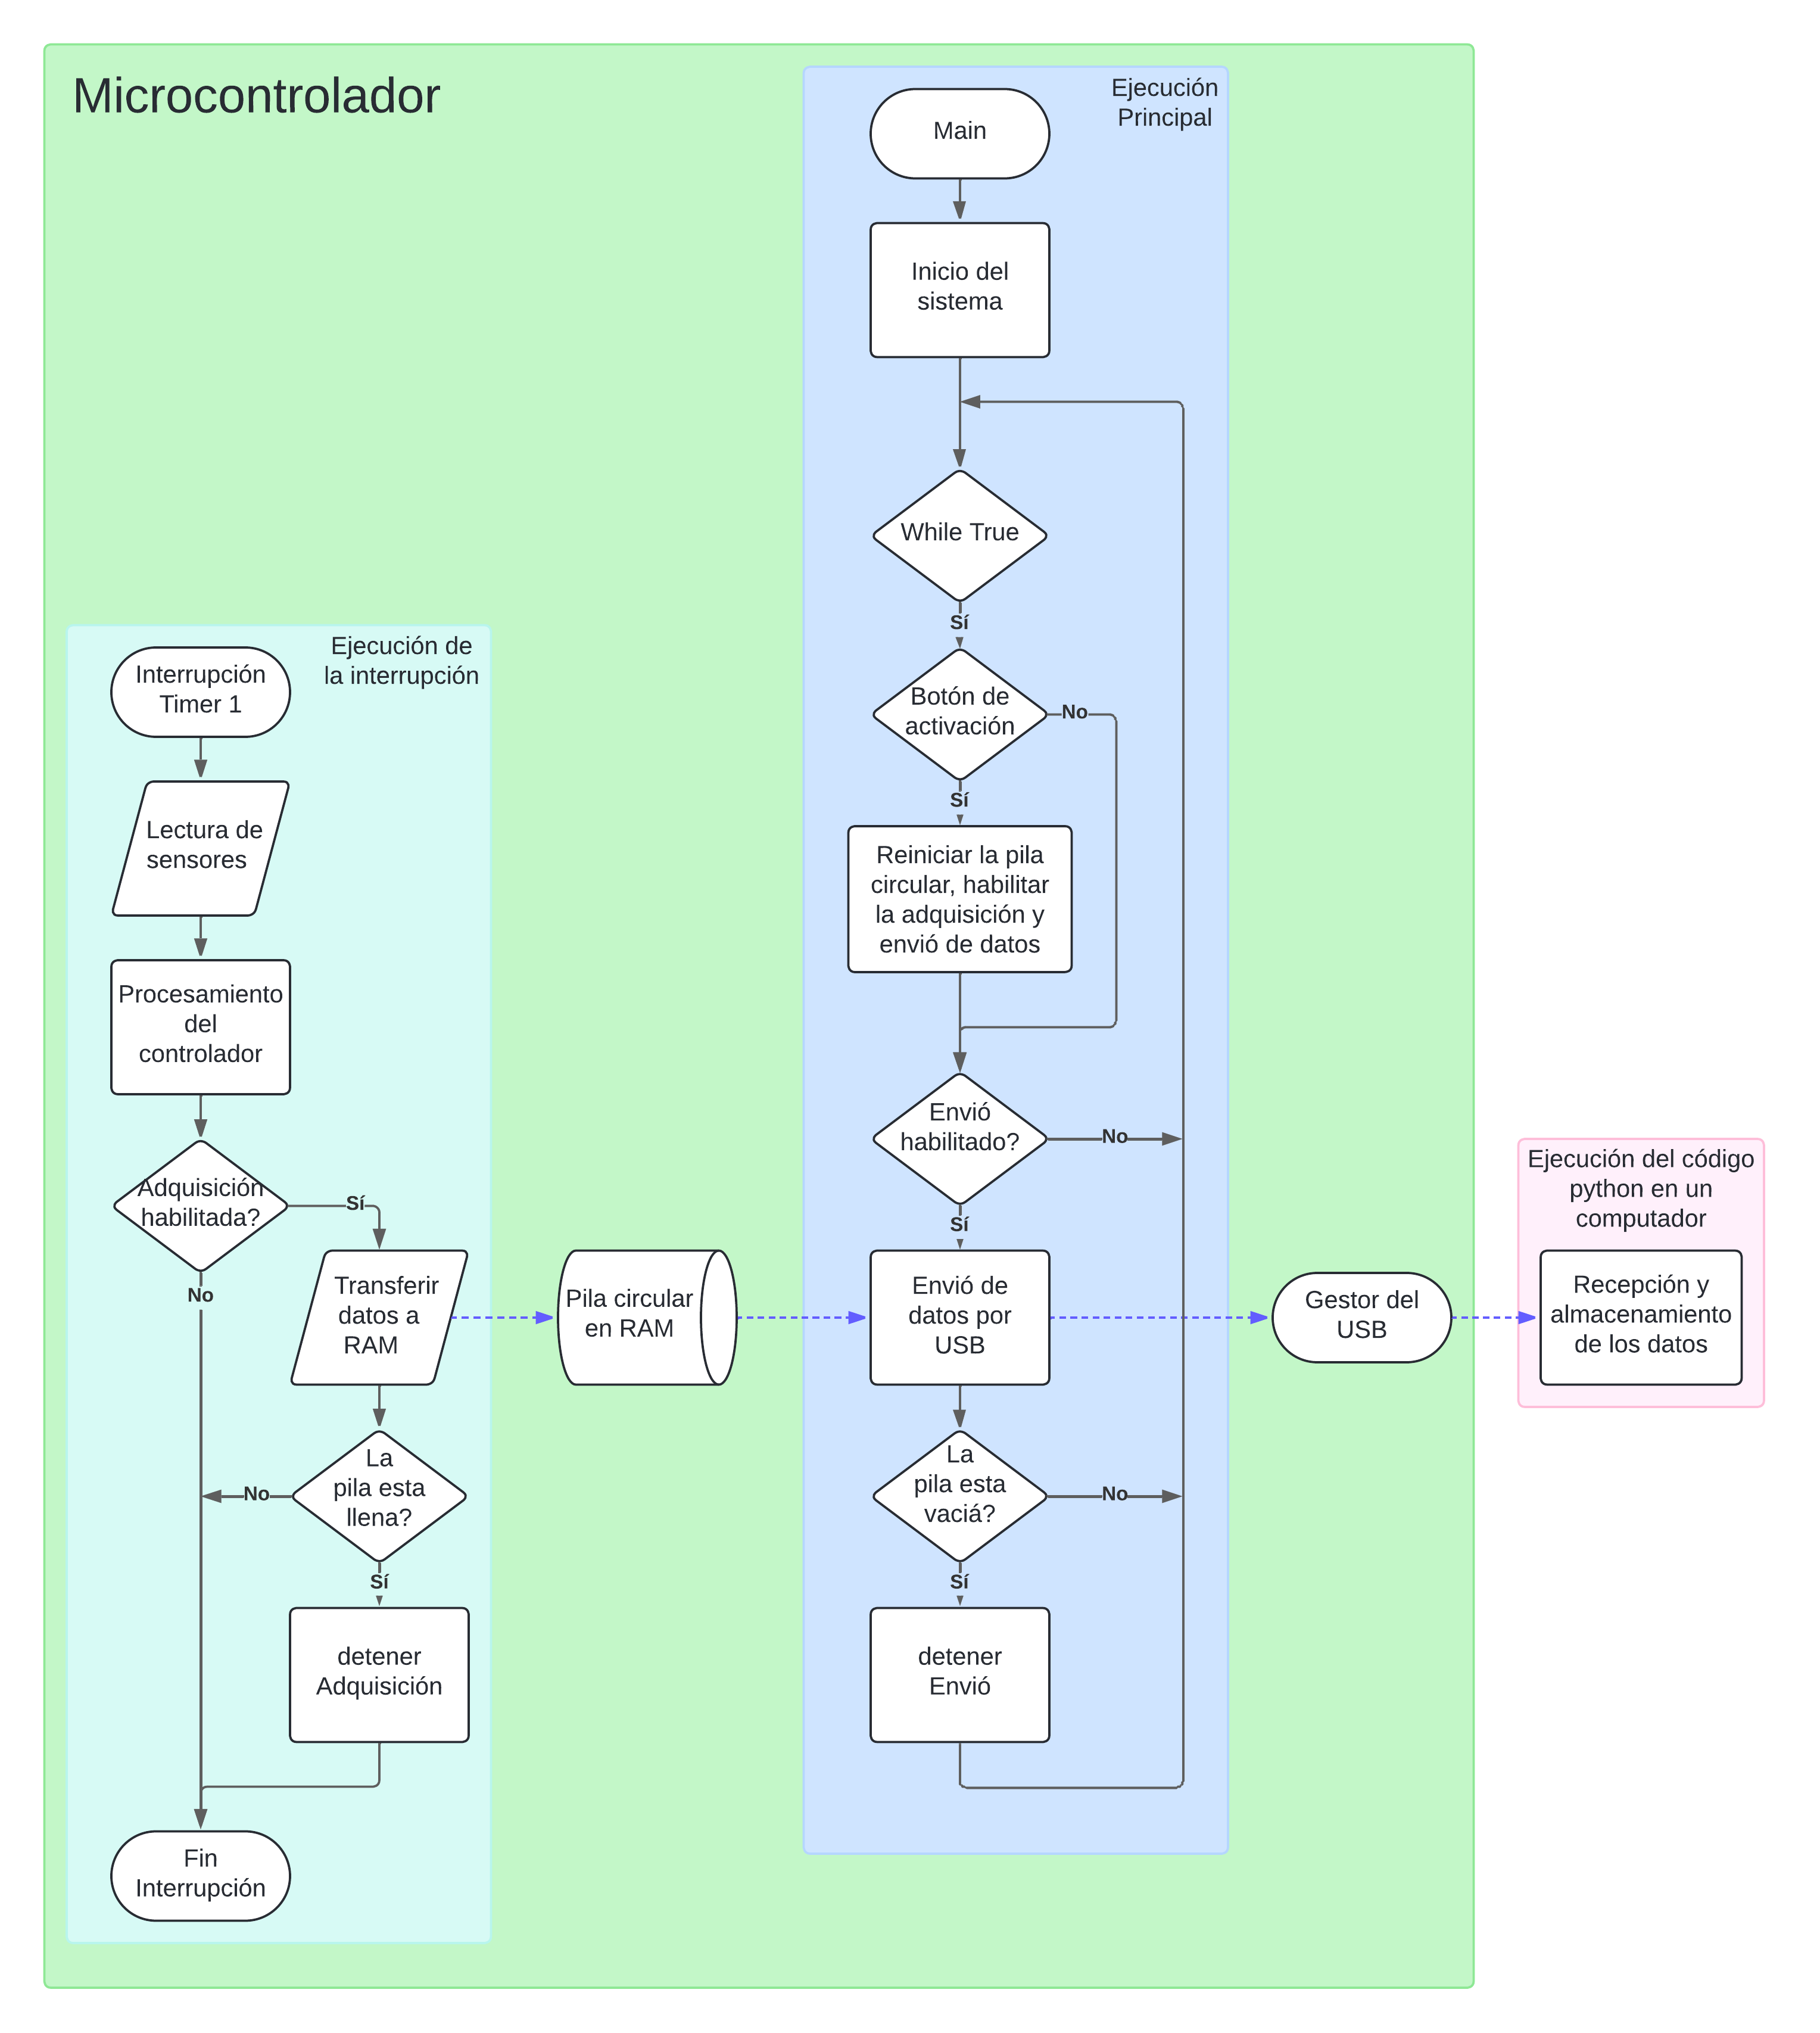
\includegraphics[width=0.76\textwidth]{imagenes/Debug USB.png}
	\caption{Diagrama de flujo adquisición de datos.}
	\label{flujo_debug}
\end{figure}
\FloatBarrier

\section{Validación de la adquisición y transformación de las mediciones de corriente}

\subsection{Validación de las mediciones de corriente}
Se validaran las mediciones de corriente adquiridas desde el microcontrolador.

\begin{figure}[ht]
	\centering
	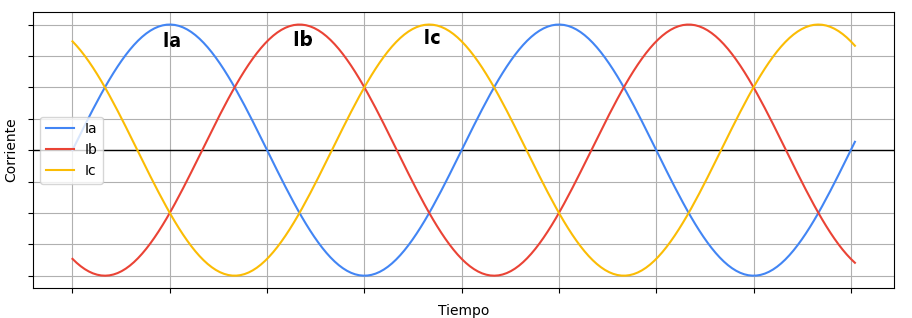
\includegraphics[width=0.8\textwidth]{imagenes/Corrientes_ABC_ideal.png}
	\caption{Corrientes ideales en un sistema trifásico equilibrado.}
	\label{corrientes_ABC_ideal}
\end{figure}
\FloatBarrier

En la figura \ref{corrientes_ABC_ideal} se representan las señales ideales de un sistema trifásico equilibrado, con las tres corrientes de fase $I_a$, $I_b$ e $I_c$, cada una de ellas con una forma senoidal pura y un desfase de $120^\circ$ entre sí.

\begin{figure}[ht]
	\centering
	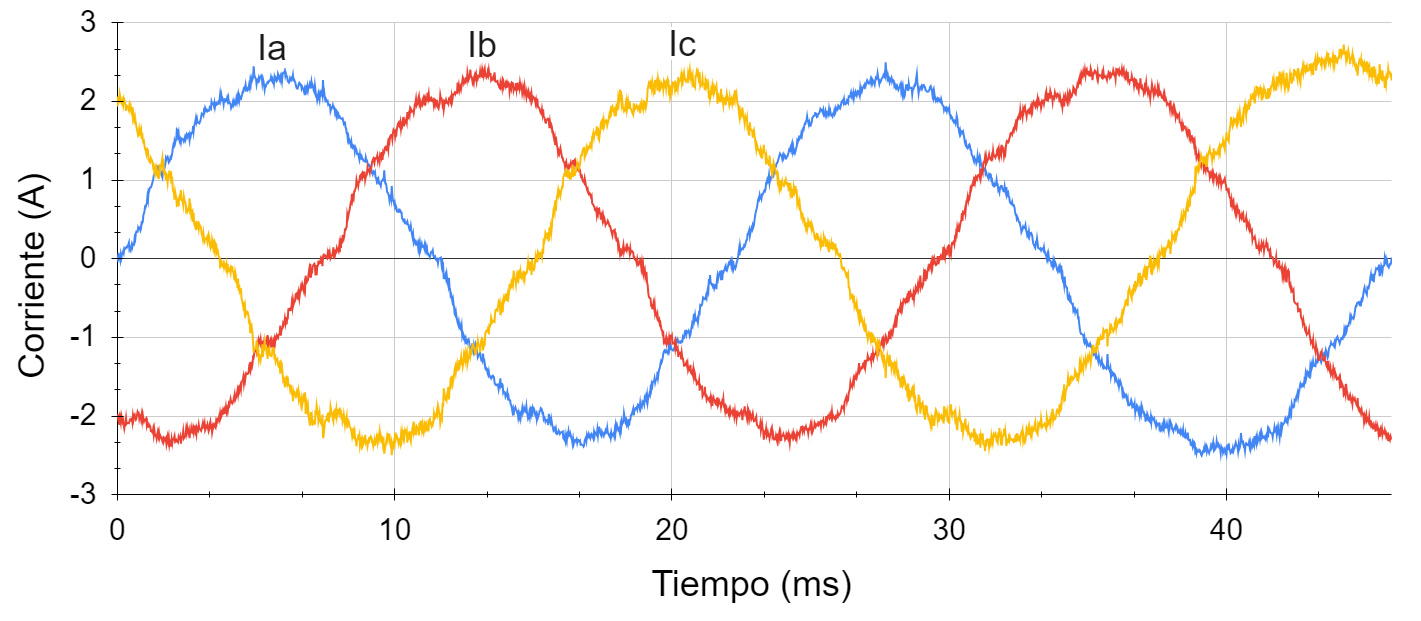
\includegraphics[width=0.8\textwidth]{imagenes/Corrientes_ABC.png}
	\caption{Corrientes medidas en el sistema trifásico.}
	\label{corrientes_ABC}
\end{figure}
\FloatBarrier

En la figura \ref{corrientes_ABC} se pueden apreciar las corrientes de fase, las cuales presentan una cantidad significativa de ruido, aun cuando internamente pasan por un filtro complementario con una frecuencia de corte $f_W=12000Hz$, pero mantienen un comportamiento sinusoidal con el desfase de $120^\circ$ entre señales, como es característico de un sistema trifásico equilibrado. pero la cantidad de ruido podría indicar que seria necesario disminuir la frecuencia de corte en el filtro complementario o agregar un filtro pasivo en el circuito.

\newpage
\subsection{Validación de la transformada de Clarke}

Se validara los resultado a la salida de la transformada de Clarke en el microcontrolador.

\begin{figure}[ht]
	\centering
	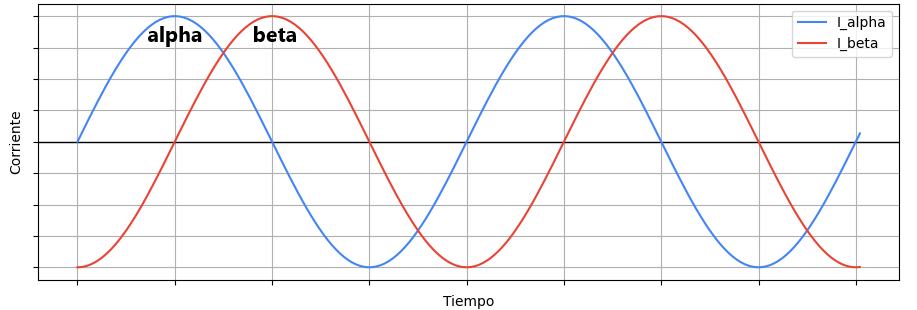
\includegraphics[width=0.8\textwidth]{imagenes/Corrientes_AlphaBeta_ideal.png}
	\caption{Corrientes ideales en el plano $\alpha\beta$.}
	\label{corrientes_alpha_beta_ideal}
\end{figure}
\FloatBarrier

En la figura \ref{corrientes_alpha_beta_ideal} se representan las corrientes ideales en el plano $\alpha\beta$, con las formas senoidales puras con un desfase de $90^\circ$ entre sí.

\begin{figure}[ht]
	\centering
	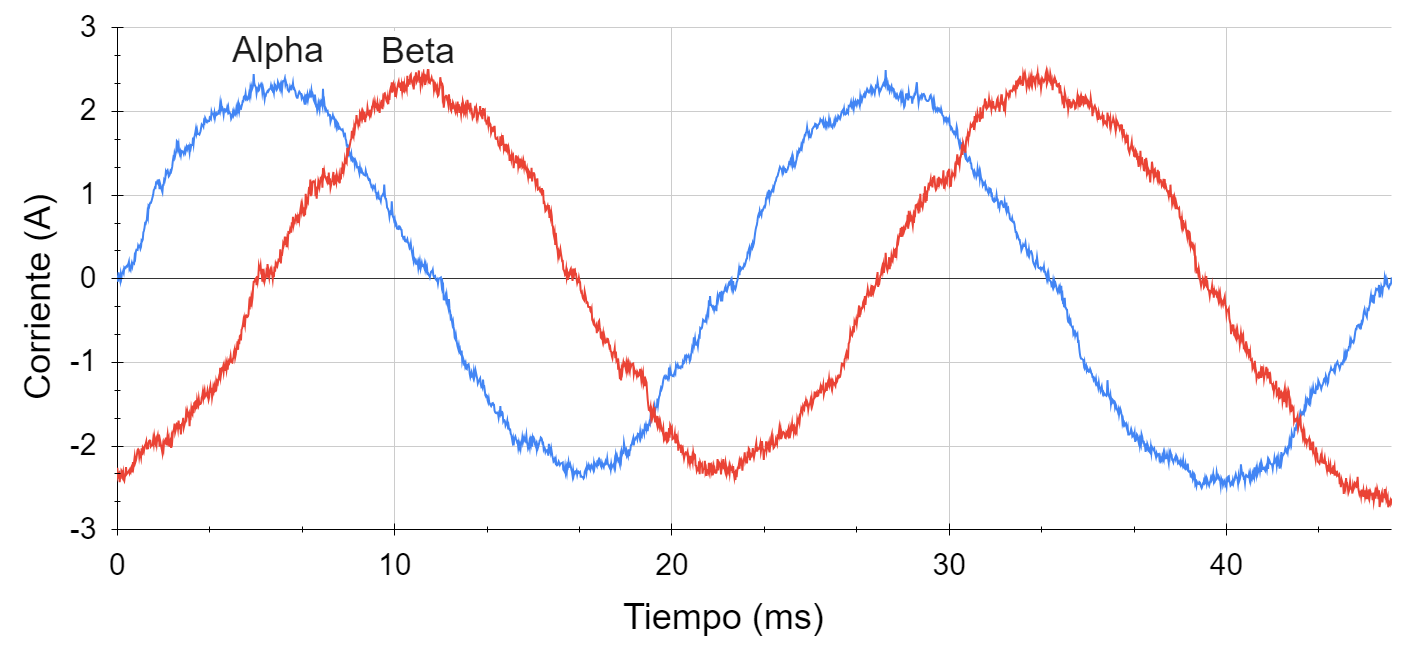
\includegraphics[width=0.8\textwidth]{imagenes/Corrientes_AlphaBeta.png}
	\caption{Corrientes medidas en el plano $\alpha\beta$.}
	\label{corrientes_alpha_beta}
\end{figure}
\FloatBarrier

En la figura \ref{corrientes_alpha_beta} se pueden apreciar como las corrientes $\alpha\beta$ reflejan el ruido presente en las mediciones de los sensores de corriente, pero mantienen un comportamiento esperado a la salida de la transformada de Clarke con las dos señales sinusoidal con el desfase de $90^\circ$ entre señales, como es característico.

\newpage
\subsection{Validación de la transformada de Park}

Se validara los resultado a la salida de la transformada de Park en el microcontrolador.

\begin{figure}[ht]
	\centering
	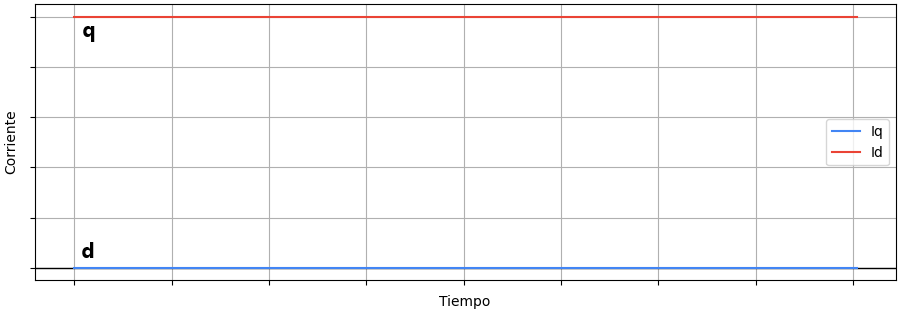
\includegraphics[width=0.8\textwidth]{imagenes/Corrientes_dq_ideal.png}
	\caption{Corrientes ideales en el plano $dq$.}
	\label{corrientes_dq_ideal}
\end{figure}
\FloatBarrier

En la figura \ref{corrientes_dq_ideal} se representan las corrientes ideales en el plano $dq$, donde lo ideal, es que la corriente directa tenga un valor de cero, para mantener la eficiencia del sistema, mientras que solo la corriente de cuadratura tiene un valor distinto a cero.

\begin{figure}[ht]
	\centering
	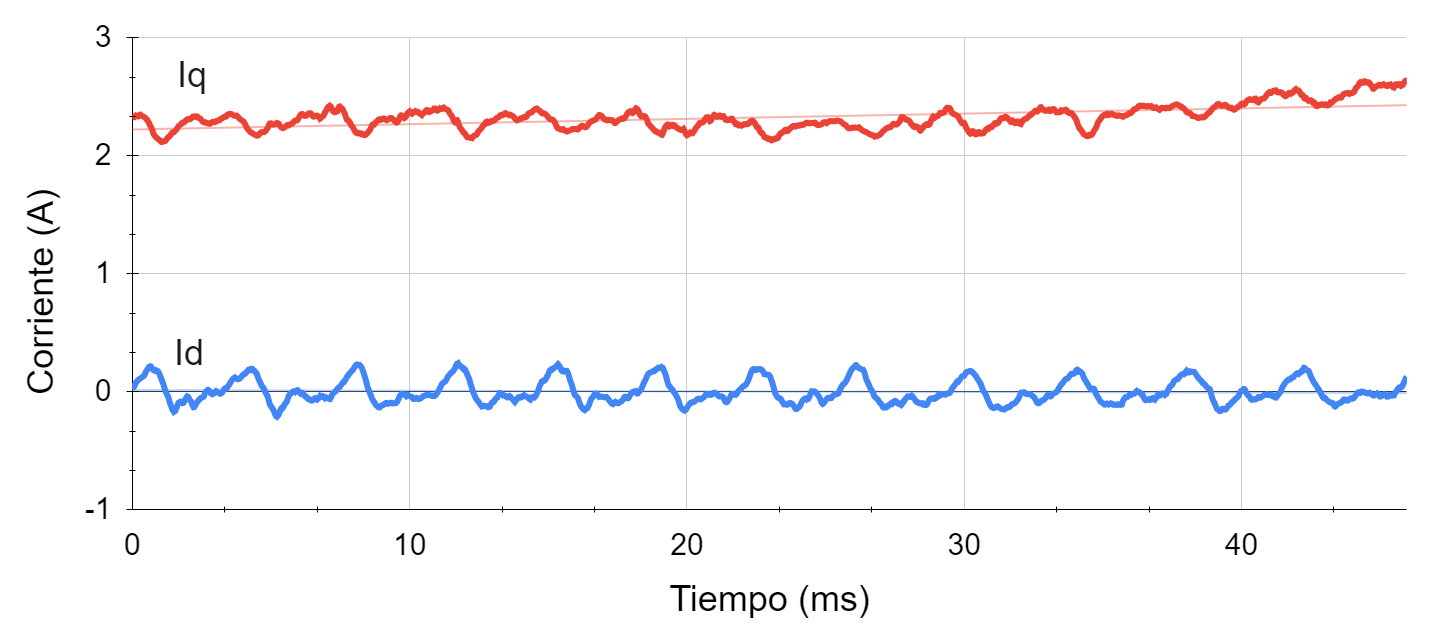
\includegraphics[width=0.8\textwidth]{imagenes/Corrientes_dq.png}
	\caption{Corrientes medidas en el plano $dq$.}
	\label{corrientes_dq}
\end{figure}
\FloatBarrier

En la figura \ref{corrientes_dq} se pueden apreciar como las corrientes $dq$ presenta una menor cantidad de ruido gracias a que su filtro complementario esta ajustado para una frecuencia de corte de $f_W=800Hz$, aunque igualmente presentan ciertas deformaciones y e inestabilidad con un patron aparentemente constante, pero en términos generales mantienen aproximadamente el comportamiento esperado a la salida de la transformada de Park.

\newpage
\section{Validación de los Controladores PI}
En esta validación se busca comprobar si los controladores PI de velocidad y corriente son capaces de mantener sus setpoints. Las pruebas se realizaron de forma estática, aplicando una carga ligera sobre el motor y capturando datos durante este proceso.

\subsection{Validación del controlador de velocidad}
Para la validación, se aplicó un setpoint de 116.8 RPM utilizando uno de los potenciómetros disponibles.

\begin{figure}[ht]
	\centering
	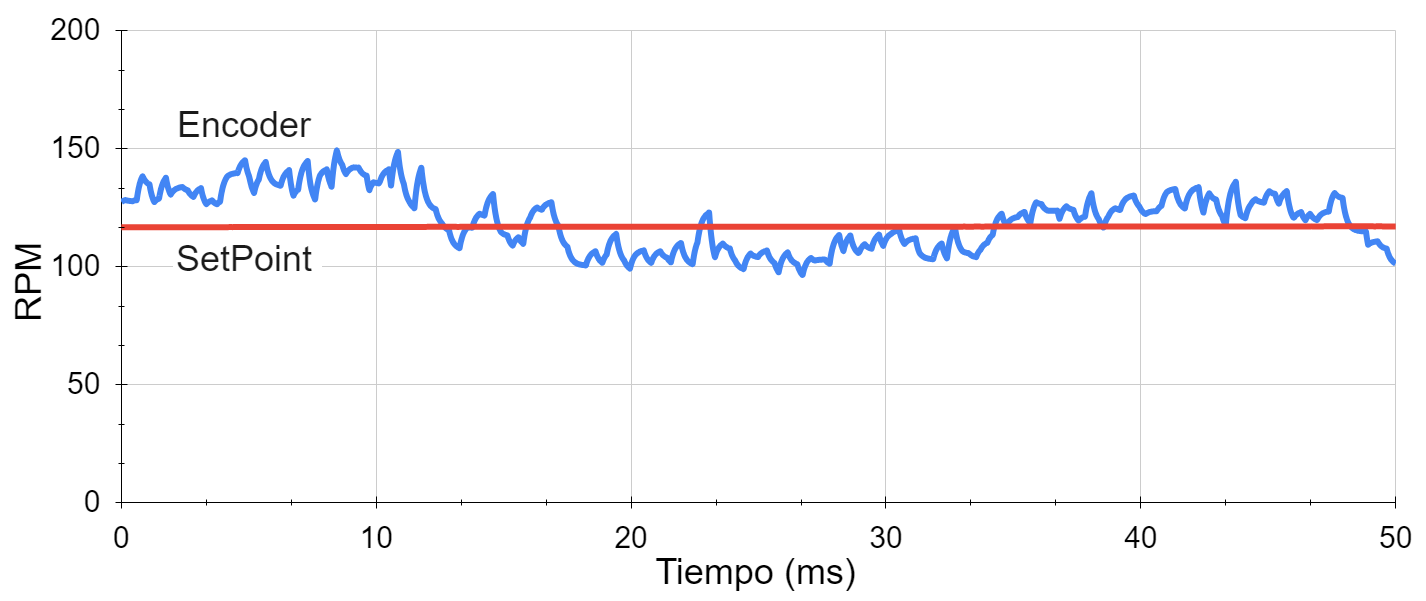
\includegraphics[width=0.8\textwidth]{imagenes/CV.png}
	\caption{Velocidad medida por el encoder y setpoint de velocidad.}
	\label{velocidad_encoder}
\end{figure}
\FloatBarrier

En la Figura \ref{velocidad_encoder}, se observa que la velocidad medida por el encoder sigue adecuadamente el setpoint establecido de 116.8 RPM. A pesar de ligeras oscilaciones, el controlador de velocidad mantiene el régimen deseado, demostrando su capacidad para alcanzar y mantener el setpoint bajo condiciones de carga estática.

\newpage
\subsection{Validación del controlador de corriente}

\begin{figure}[ht]
	\centering
	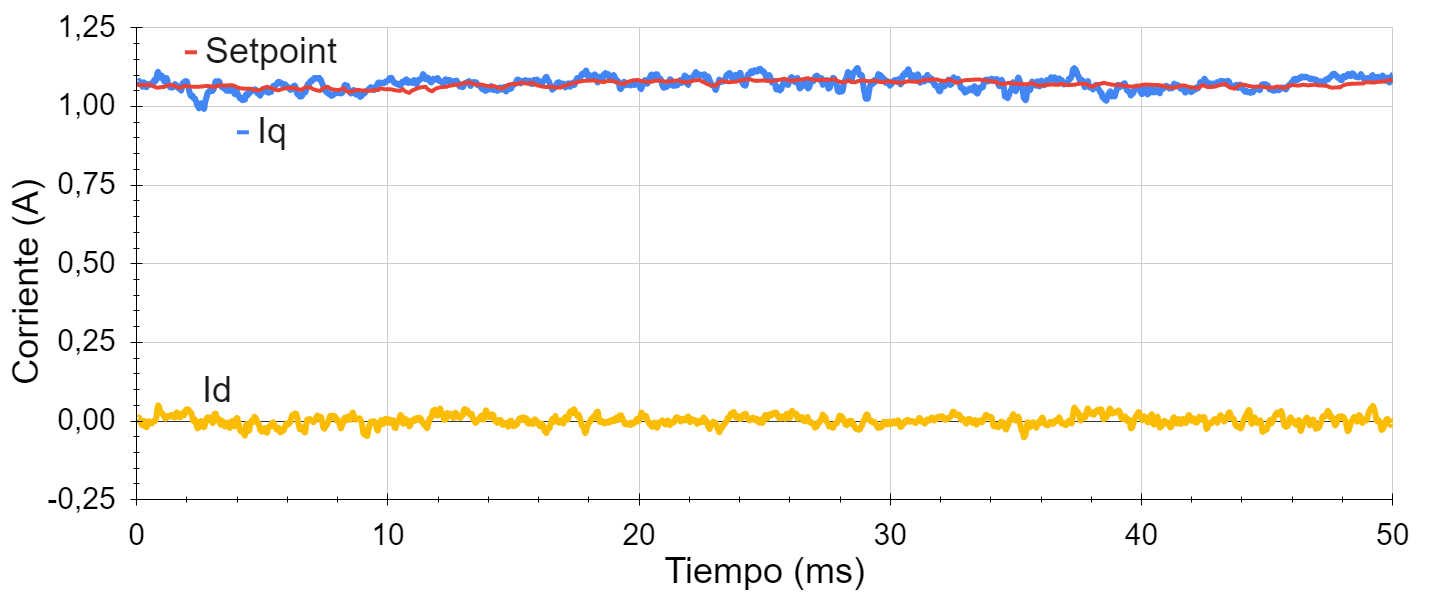
\includegraphics[width=0.8\textwidth]{imagenes/CV_CC.png}
	\caption{Corrientes medidas en el plano $dq$.}
	\label{cont_corrientes_dq}
\end{figure}
\FloatBarrier

Como se muestra en la Figura \ref{cont_corrientes_dq}, las corrientes en el plano $dq$ indican que el controlador de corriente logra mantener la corriente de cuadratura ($I_q$) cercana al valor de referencia proporcionado por el controlador de velocidad, mientras que la corriente directa ($I_d$) se mantiene próxima a cero. Esto evidencia que el controlador de corriente regula eficazmente las corrientes según los setpoints establecidos.

\begin{figure}[ht]
	\centering
	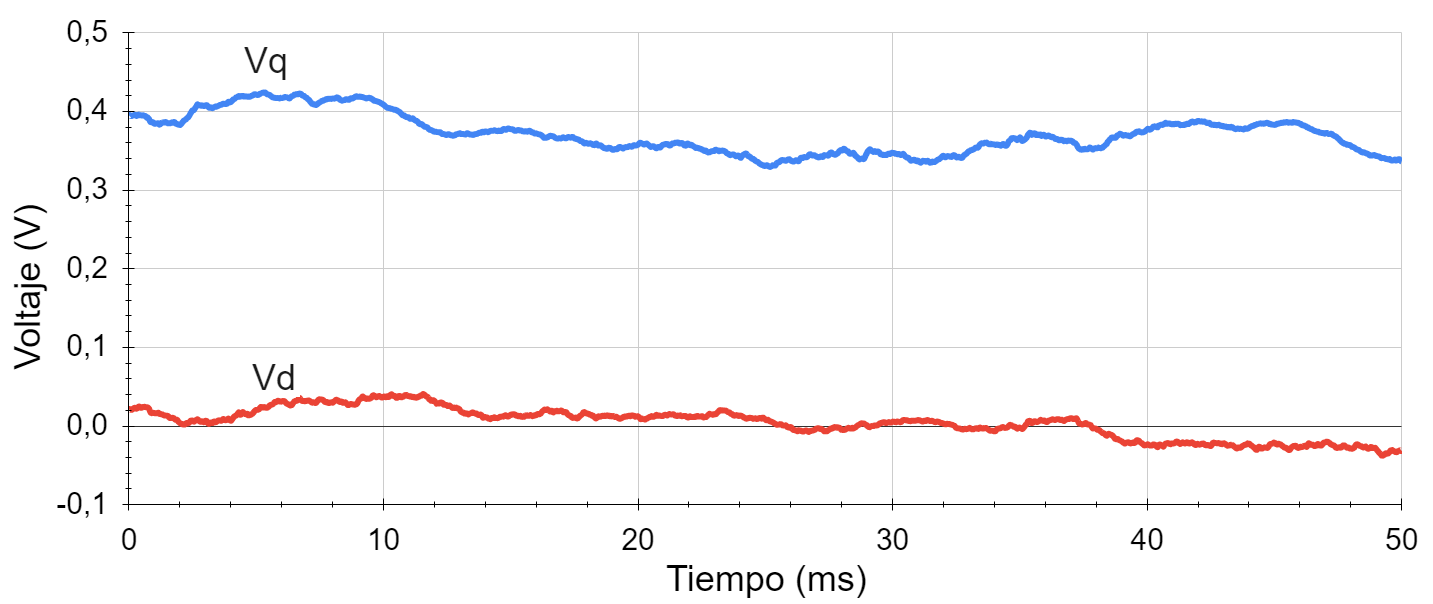
\includegraphics[width=0.8\textwidth]{imagenes/CC_DQ.png}
	\caption{Voltajes en el plano $dq$.}
	\label{voltajes_dq}
\end{figure}
\FloatBarrier

Además, la Figura \ref{voltajes_dq} presenta los voltajes en el plano $dq$, donde se aprecia que las tensiones generadas están dentro de los valores esperados para mantener las corrientes deseadas. Esto corrobora que el controlador de corriente responde adecuadamente a las demandas del sistema, contribuyendo al correcto desempeño del motor bajo condiciones de carga.

\newpage
\section{Validación señales del SVM}

Para validar el funcionamiento del modulador por vector espacial (SVM), se realizaron pruebas virtuales aplicando diferentes valores de tensión de referencia $V_{\text{ref}}$ al SVM para observar su comportamiento. Durante estas pruebas, se utilizó un analizador lógico para capturar las señales PWM generadas por el microcontrolador. En la captura presentada, se aisló un ciclo completo del PWM donde se puede apreciar de forma clara la secuencia de activación correspondiente al sector 1.

\begin{figure}[ht]
	\centering
	\includegraphics[width=0.9\textwidth]{imagenes/señales timer.png}
	\caption{Señales del timer.}
	\label{señal_timer}
\end{figure}
\FloatBarrier

En la Figura \ref{señal_timer}, se observan las señales PWM correspondientes a las tres fases generadas por el microcontrolador. La secuencia de activación muestra que el SVM implementado sigue correctamente el patrón teórico esperado para el sector 1, evidenciando una conmutación precisa y sincronizada de los transistores del inversor. Esto confirma que el SVM está modulando adecuadamente las señales PWM para generar los vectores de tensión requeridos.

\newpage
\chapter*{Comentarios y Conclusiones}
\addcontentsline{toc}{chapter}{Comentarios y Conclusiones}

\newpage
\addcontentsline{toc}{chapter}{Bibliografía}
\printbibliography

\newpage
\addcontentsline{toc}{chapter}{Anexos}

\chapter*{Anexo A}
\addcontentsline{toc}{section}{Anexo A}

\end{document}
